\chapter{Modeling Cyber-Insurance }
\label{chp:modelingCyberInsurance} 


\section{Network Formation}


In many scenarios agents seeks to create networks in order to directly benefit from each other. The established links might represent companies out sourcing part of their manufacturing, or cooperative agreements in the development of new software products. In addition to increase the trade-off, each of the established links represents risk of being a victim of cascading failures. The intuitive example is the spread of epidemic diseases, also  (node failures of a power grid and) financial contagion such as the one back in 2008 was a result of cascading failures. Strategic network formation using cyber-insurance can be used to prevent such situation in addition to increase the overall payoff of participants in a clustered network.


When deciding whether to establish connection to a neighbour agent, the payoff has to be a balance between the expected earnings and the risk of the other party failing to complete the transaction. This is the reason why we seek to only download content from trusted peers and outlaw MC-gangs are consistently skeptical to enter into new agreements despite promising increased earnings, since the risk of undercover police are too high. 


In the paper \cite{contagion}, they come up with some interesting results regarding network formation games. 
They set up a game where the nodes benefit from direct links, but these links also expose them for risk. 
Each node gains a payoff of  $a$ per link it establishes, but it can establish a maximum of $\delta$ links.
A failure occur at a node with probability $q$, and propagates on a link with probability $p$. If a nodes fail, it will receive a negative payoff of $b$, no matter how many links it has established.

The results from their model shows a situation where clustered graphs achieve a higher payoff when connected to trusted agents, compared to when connecting with random nodes. Unlike in anonymous graphs, where nodes connect to each other at random, nodes in these graphs share some information with their neighbours, which is used when deciding whether to form a link or not. 
To further explain these results, they show that there exists a critical point, called phase transition, which occurs when nodes have a node degree of $1/p$. 
At this point a node gets a payoff of $a/p$, to further increase the payoff the node needs to go into a region with significantly higher failure probability. 
Because once each node establish more than $1/p$ links, the edges which propagates risk, will with high probability form a large cluster. Which results in a rise in probability of node failure, and reduces the overall wellfare.
From this the paper say that when the minimum welfare exceeds 
$(1+f(\delta)*a/p)$
we have reached super critical payoff. Otherwise it is called sub-critical payoff. 
Further they show that the only possible way of ending up with supercritical payoff, is by forming clustered networks consisting of cliques with slightly more than $1/p$ nodes. 
If the nodes form an anonymous market, random linking, they can only get sub-critical payoff. 
In other words, if the nodes can choose who they connect with, and by doing so, creating trusted clustered markets, they can achieve a higher payoff, by exceeding the critical node degree point. But in random graphs, this is not possible. 


Inspired by this model, we created a model which shields light on how cyber-insurance can be used in network formation to prevent cascading failures and increase an agents payoff.  



\section{Very Simple Model \label{section:verysimplemodel}}

As a starting point the model is highly simplified in order to show the concept of how cyber-insurance can be used to create an insurable topology. Through out this chapter new features will be added to the model to make it more realistic and applicable. To begin, the model is formulated as follows.
A set of $n$ agents are randomly chosen to be insured or not, as depicted in figure \ref{fig:firstmod1}. They all get their own fixed income, and by connecting to other agents they will receive a benefit resulting in higher payoff. Non-insured agents will have a risk of failure i.e. an expected cost of failure. Therefore if an insured agents chooses to connect to a non-insured agent they will also suffer from this expected cost of failure. In other words, the model follows a rule that insured agents are only willing to connect to other insured agents and non-insured agents can only connect with each other. In addition we apply the assumption that each node goes through the whole graph to decide whether to establish a connection or not. Since the decision is bidirectional, i.e. each agent must agree to establish the connection. The resulting graph will always be two fully connected cliques, one consisting of insured agents and the other of non-insured agents. 


This dichotomy represents a trusted environment for the insured nodes, because they are able to trust each other since everyone is protected from risks such as financial catastrophe. These agents will benefit from each connection without having to worry about contagious risks from the connected agents. 
An agent in the non-insured clique will also receive the aggregated benefits from the connections, however each of the connection has a probability of failure. Hence this environment is not trusted, and a decision on whether to connect always involves some risks. 

\begin{figure}[h]
\centering
\begin{subfigure}{.5\textwidth}
  \centering
  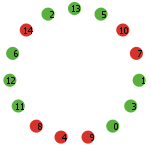
\includegraphics[width=0.4\linewidth]{../Figures/firstModelWithNoParameters1.png}
  \caption{\label{fig:firstmod1} 15 Agents randomly choosen to be either insured (green) or non-insured (red).}
\end{subfigure}
\quad
\begin{subfigure}{.46\textwidth}
  \centering
  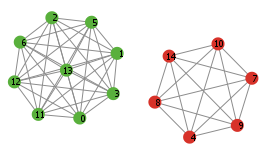
\includegraphics[width=0.8\linewidth]{../Figures/firstModelWithNoParameters2.png}
  \caption{\label{fig:firstmod2} Two clustered networks. One consisting of insured agents the other consists of non-insured.}
\end{subfigure}
\caption{\label{fig:fincont} shows how agents connects to eachother according to model described in section \ref{section:verysimplemodel}.}
\end{figure}


There are many examples of nodes needing to establish connections, one example is a firm who needs to out-source certaint tasks to remain competitive. This outsourcing involves some risks, such as, will the company deliver at the reported time, to the reported costs, what happens if they fail to deliver, if they go bankrupt etc. If the firms that are going to establish links(contracts), know that the other firms are insured, it will be easier and more secure to establish links. In this way trusted cliques can evolve. The firms benefit from connecting to other insured firms, and the insurance company can offer fair prices to the insured companies, because they know that they are in a trusted clique.
Hence this model, although very simple, shows an insurable topology where insured agents benefit from being insured. 


The model is very simplified and suffer from many limitations, among others it is too simple to reflect the dynamics of a real world scenario, where each node will have different variables with different values. In addition, each node have a complete network information i.e. the problem with information asymmetry is not taken into account. But the model is a good starting point. 

\subsection{Model with parameters}
To make the simple model more realistic, we have to create a game with parameters. The characteristics of the game is as follows: an agent can be either insured or not insured, the insured ones have to pay an insurance cost $I_{0}$. Every agent starts with a fixed income, $\alpha$, to further increase their income they have to establish links to other agents. For each link they establish they receive a payoff of $\beta$. This represents the positive network externalities of the game. A insured node has to pay a cost of $I_{l}$ for every link he establishes. The game is bidirectional, i.e. both nodes need to agree of the establishment of a link, and if both are insured, they both have to pay the cost $I_{l}$. 
Every agent who is not insured will have a risk of failure(infected, bankruptcy, or some other type of failure), this is captured with the expected risk cost $r$. Every node, insured or not who connects to a non-insured node will also suffer from this cost. The link insurance cost and the risk are negative network externalities in the game. See Table \ref{tbl:simplegamepara} for an overview of the parameters. 
\begin{table}[h]
\centering
\begin{tabular}{lc}
 \hline
  $\alpha$ - agents fixed income\\
  $\beta$ - income from establishing a direct link \\
  $I_{o}$ - cost of having insurance. \\
  $I_{l}$ - increased insurance cost per link the node establishes\\
  $r$ - expected risk cost\\
  \hline
\end{tabular}
\caption{Table showing the parameters to be used in the first model \label{tbl:simplegamepara}}
\end{table}
\subparagraph{Two agent game}
To begin analysing the game, lets consider a two-person game. In this game the strategy space of both players consist of four different strategies. They can choose to purchase insurance or not, and to establish a link or not. I.e. the different strategies are: Be insured and establish link noted as: $IL$, 
be insured and do not establish link: $I\overline{L}$. Not insured and establish link: $\overline{I}L$, and not insured and do not establish link: $\overline{IL}$. It should be noted that since the decision to establish a connection is bidirectional, both have to choose a strategy where they want to establish a link, for the link to be establishment to be successful.
Figure \ref{fig:FirstGameTheoryModel} shows the different outcomes of this game.

\begin{sidewaysfigure} % <-- HERE
\centering
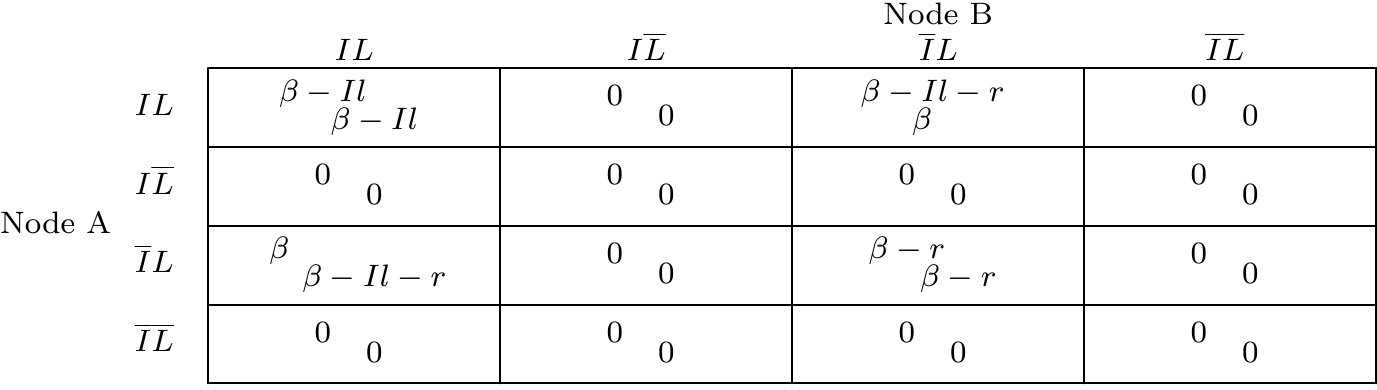
\includegraphics[width=1.0\textwidth]{../Figures/FirstGameWithParameters.png}
\caption{\label{fig:FirstGameTheoryModel} Normal form game, showing the different strategies and the payoffs  for the different outcomes. The payoff for agent A is written first, then the payoff for agent B is on the line beneath.
 An agent has a strategy space of size 4. }

\end{sidewaysfigure}


The simple game described earlier where the insured nodes form a trusted clique is what we want to achieve. 
When non-insured nodes connect to each other, they both end up with this payoff \ref{eq:notinsured payoff}. If they do not establish connection, they both receive the payoff \ref{eq:notinsured payoff2}.
\begin{equation}
U=\alpha - 2*r +\beta
\label{eq:notinsured payoff}
\end{equation}
\begin{equation}
U=\alpha - r
\label{eq:notinsured payoff2}
\end{equation}
From this equation we see that if $r>\beta$ then no connections will be made between non-insured nodes, because they would strictly prefer the payoff from not connecting.
If an insured agent connects to a non-insured one, he will end up with this payoff \ref{eq:insured-noninsured}. If he do not connect he will receive the payoff shown in \ref{eq:insured-noninsured2}.
\begin{equation}
U=\alpha - I_{0} - I_{l} - r + \beta
\label{eq:insured-noninsured}
\end{equation}
\begin{equation}
U=\alpha - I_{0}
\label{eq:insured-noninsured2}
\end{equation}
If $I_{l}+r>\beta$ the insured one will prefer not to connect, else he would prefer to establish a connection, and since the non-insured agent is always better off when connected to an insured agent, he will accept the establishment. This is easy to see when comparing the two payoffs. Payoff of connecting to an insured one: $U_{i}=\alpha - r + \beta$ is allways higher than not connecting: $U_{i}=\alpha - r$, as long as $\beta>0$.
\subparagraph{Multiple nodes}
We want our game to end up in a trusted clique of insured nodes, to achieve this we need to make sure that only insured nodes connect to each other, we want \ref{eq:insured-noninsured2} to be larger than \ref{eq:insured-noninsured}. I.e. This has to hold:
\begin{equation}
I_{l}+r>\beta
\label{eq:condition}
\end{equation}
When insured nodes connect to other insured nodes, they both end up with this payoff:
\begin{equation}
U=\alpha - I_{0} - I_{l} + \beta
\label{eq:insured-insured}
\end{equation}
To ensure that both agents will connect to each other this has to hold:
 \begin{equation}
I_{l}<\beta
\label{eq:condition2}
\end{equation}
For the game to end up as the one described earlier, where only insured nodes connect to other insured nodes, both \ref{eq:condition} and \ref{eq:condition2} has to hold, which gives us this limitation on the parameter $I_{l}$:
\begin{equation}
\beta-r<I_{l}<\beta
\label{eq:final condition}
\end{equation}
If the cost of insuring link is between these bounds, the insured nodes will only connect to other insured nodes. This holds for any number of players, because the relative change in payoff is linear and non-dependent on number of links already established. 
If the condition is fulfilled the game will end up in one or two cliques. Two cliques if the non-insured nodes connect to each other, and they do so if: $\beta>r$. 

In this model the network formation is done endogenously, and when following the limitation \ref{eq:final condition} we ensure that only insured nodes will connect, and the network ends up in a insurable network topology. 
We have neglected the information problem, because we made the assumption that all nodes can differentiate insured versus non insured nodes. This could be difficult to realize in many real world network, but in financial transactions and in software development networks, it is reasonable to assume that the parties can acquire this type of information regarding their transactional partners. And thus they solve the information asymmetry problem by them self, by requiring proof of insurance prior to establishing a connection. 
And as shown, if the insurance cost is within its needed limitations, the network will evolve endogenously, and end up with a insurable-clustered component. This is beneficial for both the insurer and the nodes.

\subparagraph{Example scenario}
By assigning values to the variables, we can show the outcome of the game in different scenarios. With the values from table \ref{tbl:simplegamevalue}, the insurance cost of establishing a link satisfies the condition in equation \ref{eq:final condition}.
If we play this game between two agents we can see the result in the normal form table \ref{fig:NFnumbers}. 
We see that the results are as we expected, insured nodes will only choose to connect with other insured nodes, they are also satisfied when not connected to each other, but this is not the social optimal outcome, and since they have complete network information, they will choose to connect to each other, because they will both achieve a higher payoff.
As we know, it does not matter if we only consider a two person game, because the change in payoffs of adding a link, is linear an independent of the agents degree, and if the insurance cost is right, it will never be beneficial for a insured node to connect to a non-insured. 

\begin{table}[h]
\centering
\begin{tabular}{lc}
 \hline
  $\alpha=10,
  \beta=10,
  I_{o}=5,
  I_{l}=3,
  r=8$\\
  \hline
\end{tabular}
\caption{Table showing the parameters and their assigned values \label{tbl:simplegamevalue}}
\end{table}

\begin{figure}[h]
\centering
\begin{tabular}{@{}c@{}}
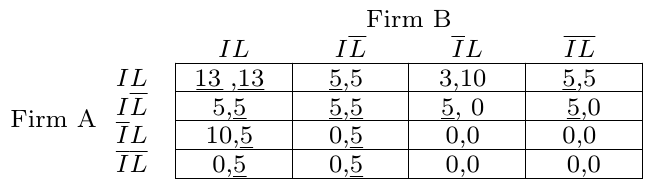
\includegraphics[width=1.0\textwidth]{../Figures/gameTheoryModel1WithNumbers.png}
\end{tabular}
\caption[Caption for LOF]{Normal form game between two agents with the parameters given in \ref{tbl:simplegamevalue}, the best response of a player to a given strategy is marked with an underscore.There are two pure nash equilibriums in this game,$IL,IL$ and $I\underline{L},I\underline{L}$. \label{fig:NFnumbers}}
\end{figure}
When setting the insurance cost: $I_{l}<\beta - r$ or $I_{l}>\beta$ we are violating the condition who ensured that only insured nodes connected to each other.If we let the insurance cost be: $I_{l}<\beta - r$, like in the table \ref{tbl:simplegamevalue2}, we will get the results shown in Figure \ref{fig:NFnumbersViolating}. There are still the same nash equilibriums, but the interesting part is the best response of an insured agent who want to establish link, when the other agent is not insured but also want to establish link. This scenario has now changed, and we see that the insured agent would agree to the link establishment, this will result in an untrusted and thus an non-insurable topology. A game with multiple agents, insured and non-insured, will end up in one fully connected network.
On the other hand, if $I_{l}>\beta$, then it is easily seen that only the non-insured will connect to each other, and the insured nodes will choose not to connect to anyone because it is to expensive.
 Therefore to ensure that only insured agents connect to each other, equation \ref{eq:final condition} has to be satisfied. 
\begin{table}[h]
\centering
\begin{tabular}{lc}
 \hline
  $\alpha=10,
  \beta=10,
  I_{o}=5,
  I_{l}=1,
  r=8$\\
  \hline
\end{tabular}
\caption{Table showing the parameters and their assigned values, the insurance cost of establishing link is now violating the equation \ref{eq:final condition} \label{tbl:simplegamevalue2}}
\end{table}

\begin{figure}[h]
\centering
\begin{tabular}{@{}c@{}}
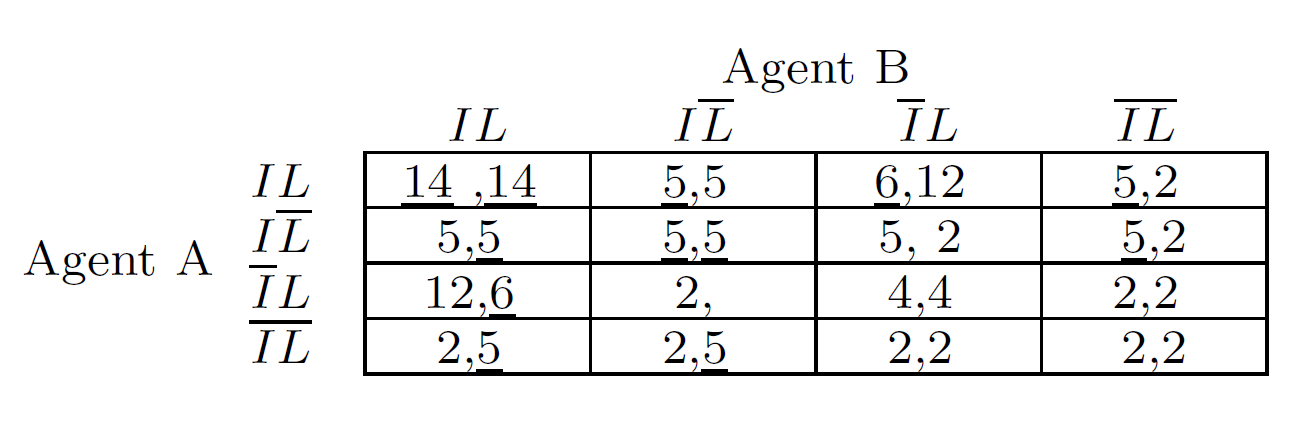
\includegraphics[width=1.0\textwidth]{../Figures/NotOptimalGameWithNumbers.png}
\end{tabular}
\caption[Caption for LOF]{Normal form game between two agents with the parameters given in table \ref{tbl:simplegamevalue2}, the best response of a player to a given strategy is marked with an underscore.There are two pure nash equilibriums in this game,$IL,IL$ and $I\underline{L},I\underline{L}$. \label{fig:NFnumbersViolating}}
\end{figure}
\subsection{Modelling network formation game}
To verify the result of this network formation game with multiple nodes, we performed different simulations.  The rules are as described earlier, when a node is considering establishing a link it chooses to do so if the payoff it will receive is larger than the payoff he already poses, and the decision is bilateral. 
In the simulator a node is insured with a probability, $p$. The network formation is performed by selecting two random nodes, not neighbouring each other, then both nodes checks if they would prefer to establish a connection or not. This selection is repeated until the network are fully connected or no more nodes are willing to establish new connections.
By selecting nodes at random and checking if both of them would like to connect to each other, we relax the assumption of full network information, because now nodes only get to know if another node is insured or not, by asking them.
\subparagraph{Simulation of game with optimal parameters}
\begin{figure}[h]
\centering
\begin{subfigure}{.5\textwidth}
  \centering
  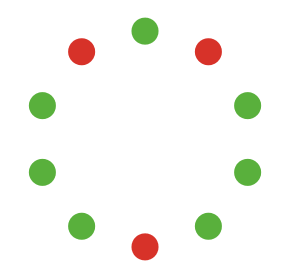
\includegraphics[width=0.4\linewidth]{../Figures/FirstSimulationStart.png}
  \caption{\label{fig:firstsimulationstart} Ten nodes randomly, with probability 0.5, chosen to be either insured (green) or non-insured (red.}
\end{subfigure}
\quad
\begin{subfigure}{.46\textwidth}
  \centering
  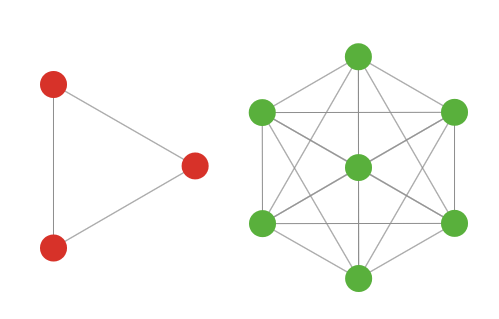
\includegraphics[width=0.8\linewidth]{../Figures/FirstSimulationResult.png}
  \caption{\label{fig:firstsimulationresult} Two clustered fully connected networks. One consisting of insured agents the other consists of non-insured. The link establishment is done by following the rules described above}
\end{subfigure}
\caption{\label{fig:firstsimulation} The figure shows how ten nodes start out with no links, and then add links as long as they can increase their payoff, the result are two seperate cliques, one consisting of non-insured and the other of insured nodes.}
\end{figure}
In figure \ref{fig:firstsimulation} we see the result of a simulation with the parameters from table \ref{tbl:simplegamevalue}, with these parameters the game should end up in two cliques, one with insured nodes and another with non-insured. The result are shown in figure \ref{fig:firstsimulationresult}. Our calculations where confirmed, only insured nodes connect to each other.  
In this figure there are only included $n=10$ nodes, this is done to make the figure understandable and readable.
The same results where confirmed when performing the simulation with larger values of n, but the resulting picture was very complex and chaotic.
\subparagraph{Simulation of game with parameters violating equation \ref{eq:final condition}}
\begin{figure}[h]
\centering
\begin{subfigure}{.5\textwidth}
  \centering
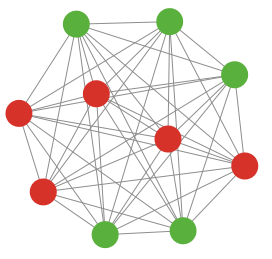
\includegraphics[width=0.4\linewidth]{../Figures/FirstSimulationViolatingResult.png}

\caption{\label{fig:SimulationViolatingA} Ten nodes insured with probability 0.5, and the parameters from table \ref{tbl:simplegamevalue2}. The link insurance cost, $I_{l}$, is violating the condition in equation \ref{eq:final condition}, and the resulting network is one clique of both insured and non-insured nodes.}
\end{subfigure}
\quad
\begin{subfigure}{0.46\textwidth}
\centering
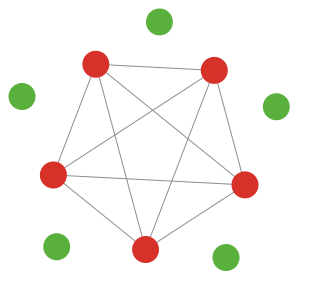
\includegraphics[width=0.4\textwidth]{../Figures/SimulationViolating2.png}

\caption{\label{fig:SimulationViolatingB} Ten nodes insured with probability 0.5, with parameters from table \ref{tbl:simplegamevalue2}, except that the link insurance cost was:, $I_{l}=11>\beta$. This resulted in a clique of only non-insured nodes. }
\end{subfigure}
\caption{\label{fig:SimulationViolating} The figure shows the two possible scenarios that violates the equation \ref{eq:final condition}, \ref{fig:SimulationViolatingA} shows the result when $I_{l}<\beta-r$ and \ref{fig:SimulationViolatingB} shows the result when $I_{l}>\beta$.}
\end{figure}

In this simulation, the cost of insuring a link where violating the equation \ref{eq:final condition}. The result can be seen in figure \ref{fig:SimulationViolating}.  In figure \ref{fig:SimulationViolatingA} we see the result when $I_{l}<\beta-r$, the result is one clique of both insured and non-insured nodes . In figure \ref{fig:SimulationViolatingB} the insurance cost is $I_{l}>\beta$, and as we see only non-insured nodes connect to each other, because the insurance cost per link cost more than the benefit gained from connecting to a new node, so the insured ones choose not to connect to any one. 

\subsection{Game with maximum node degree and bonus}
In this model we introduce a maximum node degree per node, and a payoff bonus when reaching this level. This is done to make a more applicable model in certain scenarios. For example, lets consider a software firm who want to develop a product. However, they do not have the required resources or knowledge to complete the product. They will need help from other firms, because they can deliver the desired knowledge or resources. When the product is finished the firm get paid, but not before, to finish the product they need to cooperate with other firms.
To model this scenario we added a bonus $\gamma$, which represents the payoff when a node reach their desired number off established connections, i.e. their maximum node degree($m$). Except from this fact the game is as before, nodes connect to other nodes if they can reach a higher payoff by doing so. 



\subsubsection{Four different scenarios}
To further analyze this model, lets take a closer look on the four different scenarios of the game, a insured node wants to connect to another insured node, insured tries to connect to a non-insured node, non-insured tries to connect to another non-insured node, and non-insured who tries to connect to a insured node.
\subparagraph{Insured to insured}
When an insured node tries to connect to another insured node, the node will do so if he can increase his payoff. 
Let $U_{i}$ denote the payoff of a node with node-degree $i$. When adding a link the payoff the node receives is as follows:
\begin{equation}
    U_{i+1}= 
\begin{cases}
    \alpha + \beta - I_{0} - I_{l},& \text{if } i = 0\\
    U_{i}+\beta -I_{l},& \text{if }  i>0\\
    U_{i}+\beta -I_{l}+\gamma,& \text{if } i=m
    
\end{cases}
\label{eq:itoi}
\end{equation}
For insured nodes to connect to each other, $U_{i+1} > U_{i}$. This model is very similar to the earlier model, but we need to take the received bonus when reaching $m$ into consideration.
We model this by adding, the bonus divided on the current degree, in the decision process of establishing link or not. 
\begin{eqnarray}
U_{i}+\beta-I_{l}+\frac{\gamma}{m-i}&>U_{i} \nonumber \\ 
\beta-I_{l}+\frac{\gamma}{m-i}&>0 \nonumber \\ 
\llap{$\rightarrow$\hspace{50pt}} \beta+\frac{\gamma}{m-i}&>I_{l} 
\label{eq:itoi2}
\end{eqnarray}
It should be noted that the actual bonus is not added to the current payoff before the node reach the maximum degree, as shown in equation \ref{eq:itoi}. The equation $\frac{\gamma}{ m-i}$ reflects the expected payoff from taking the risk of establishing a connection. This value increases linearly according to how close you are to reaching $m$.
In this way the model will change from the former models, because now the nodes have more incentive to connect to other nodes, and in some scenarios they will be willing to take the risk of connecting to a non-insured node that they would not have done before, due to the expected bonus. I.e. we insert some risk, because it is not certain that the nodes will obtain enough links, and if not, they will not receive their bonus, but they have already connected to the nodes.

\subparagraph{Insured connect to non-insured}
The payoff the insured node receives in this scenario is as follows:
\begin{equation}
    U_{i+1}= 
\begin{cases}
    \alpha + \beta - I_{0} - I_{l} -r,& \text{if } i = 0\\
    U_{i}+\beta -I_{l}-r,& \text{if }  i>0\\
    U_{i}+\beta -I_{l}-r+\gamma,& \text{if } i=m
\end{cases}
\label{eq:itonoti}
\end{equation}
To establish a connection from an insured node to a non-insured one, this has to hold:
\begin{eqnarray}
U_{i}+\beta-I_{l}-r+\frac{\gamma}{m-i}&>U_{i} \nonumber \\ 
\beta-I_{l}-r+\frac{\gamma}{m-i}&>0 \nonumber \\ 
\llap{$\rightarrow$\hspace{50pt}} \beta+\frac{\gamma}{m-i}-r&>I_{l} 
\end{eqnarray}
\subparagraph{Non-insured to non-insured}
When a non-insured node connect to another not-insured node this is the payoff they receive:
\begin{equation}
    U_{i+1}= 
\begin{cases}
    \alpha + \beta -r,& \text{if } i = 0\\
    U_{i}+\beta -r,& \text{if }  i>0\\
    U_{i}+\beta -r +\gamma,& \text{if } i=m
\end{cases}
\label{eq:noitonoti}
\end{equation}
To establish the connection this equation has to hold:
\begin{eqnarray}
U_{i}+\beta-r+\frac{\gamma}{m-i}&>U_{i} \nonumber \\ 
\beta-r+\frac{\gamma}{m-i}&>0 \nonumber \\ 
\llap{$\rightarrow$\hspace{50pt}} \beta+\frac{\gamma}{m-i}&>r
\end{eqnarray}
\subparagraph{Non-insured to insured}
\begin{equation}
    U_{i+1}= 
\begin{cases}
    \alpha + \beta,& \text{if } i = 0\\
    U_{i}+\beta,& \text{if }  i>0\\
    U_{i}+\beta +\gamma,& \text{if } i=m
\end{cases}
\label{eq:noitoti}
\end{equation}
As we see, this is a strictly increasing function, and thus a non-insured will always connect to an insured node if given the option, and as long as $\beta$ is positive, but this is given in the rules of the model.

\subparagraph{Limitations to ensure a clique of only insured}
We are interested in finding insurable topologies, one candidate is a clique consisting of only insured nodes. By analyzing the different scenarios above we can find limitations on the cost of insuring a link, that will force the network formation game to end up in an insurable clique.
We know that an insured node would want to connect to another insured node if the equation \ref{eq:itoi2} is satisfied. 
In the equation we see that the expected bonus per established link is increasing, i.e. if an insured node of degree zero is willing to connect to another insured node, then every node with a degree higher than zero also would like to connect to another insured node. Thus to ensure that insured nodes connect to each other this equation has to hold:
\begin{equation}
\beta+\frac{\gamma}{m}>I_{l}
\label{eq:conditionitoi}
\end{equation}
We also want to ensure that insured nodes never establishes links with non-insured nodes, from \ref{eq:itonoti} we see that this has to hold:
\begin{equation}
\beta+\frac{\gamma}{m-i}-r < I_{l}
\label{eq:conditionitonoti}
\end{equation}
This can be simplified, we know the insured nodes with degree $m-1$ get the highest expected bonus when establishing a new link, i.e. if we can ensure that nodes with this degree do not establish links to non-insured nodes, we also know that every node with degree less than $m-1$ will not establish links to non-insured nodes. From this we get the equation:
\begin{eqnarray}
\beta+\frac{\gamma}{m-(m-1)}-r&<I_{l} \nonumber\\
\llap{$\rightarrow$\hspace{50pt}} \beta+\gamma-r&<I_{l}
\label{eq:condition-i-to-noti}
\end{eqnarray}
From the equations \ref{eq:conditionitoi} and \ref{eq:conditionitonoti} we get this final limitation on the link insurance cost:
\begin{equation}
\beta+\gamma-r<I_{l}<\beta+\frac{\gamma}{m}
\label{eq:final-insurance-clique-condition}
\end{equation}
An important fact about this limitation is to make it possible for the game to end up in an insurable topology equation \ref{eq:noinsuredcliqueconditon} has to be satisfied. As we see from the equation, if the risk to bonus ratio gets to small it gets more and more unlikely to ensure an insurable topology. If we think about a real world scenario where you get a bonus for establishing a fixed number of equations, you would be more willing to take a risk if the possible reward of doing so is large, this is what this equation express. 
\begin{eqnarray}
\gamma-r &<\frac{\gamma}{m}\nonumber \\
1-\frac{r}{\gamma}&<\frac{1}{m} \nonumber \\
\llap{$\rightarrow$\hspace{50pt}}1-\frac{1}{m}&<\frac{r}{\gamma}
\label{eq:noinsuredcliqueconditon}
\end{eqnarray}

\subsubsection{Simulations}
We simulate how networks form when the conditions from equation \ref{eq:final-insurance-clique-condition} are met, and what happens when they are not. In addition we use the simulation to look at the consequences with regards to the payoff, when the required number of connections aren't met. 

\subparagraph{Conditions are met}
First we simulate a network formation game when the link insurance cost satisfied the equation \ref{eq:final-insurance-clique-condition}. 
\begin{table}[h]
\centering
\begin{tabular}{lc}
 \hline
  $\alpha=10,
  \beta=10,
  I_{o}=5,
  I_{l}=9,
  r=8,
  \gamma=5,
  m=5
  $
  \\
  \hline
\end{tabular}
\caption{Parameters used in simulation \label{tbl:maxdegrevalues}}
\end{table}
\begin{figure}[h]
\centering
  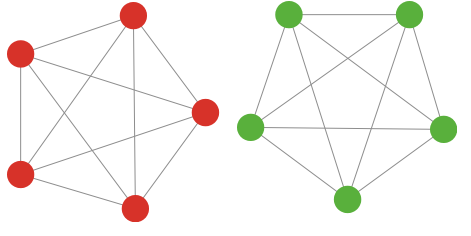
\includegraphics[width=0.8\linewidth]{../Figures/BonusGameInsuredClique.png}
  \caption{\label{fig:bonusoptimal} Two clustered fully connected networks, created by simulating with the parameters from table \ref{tbl:maxdegrevalues} One consisting of insured agents the other consists of non-insured. }
\end{figure}
As we see in figure \ref{fig:bonusoptimal} the results where as expected, the cost of insuring a link satisfied the conditions found earlier and thus the result where two cliques, one consisting of only insured and the other of non-insured nodes.

\subparagraph{Conditions are not met}
If we change the link insurance cost, so it is just below the limit, $I_{l}=6$, the result is quite different as depicted in figure \ref{fig:bonusviolating}. Here we see that eventhough non-insured nodes can fail and accumulate negative payoff, some of the insured nodes have taken a risk by connecting to one non-insured node to receive their bonus. 

\begin{figure}[h]
\centering
  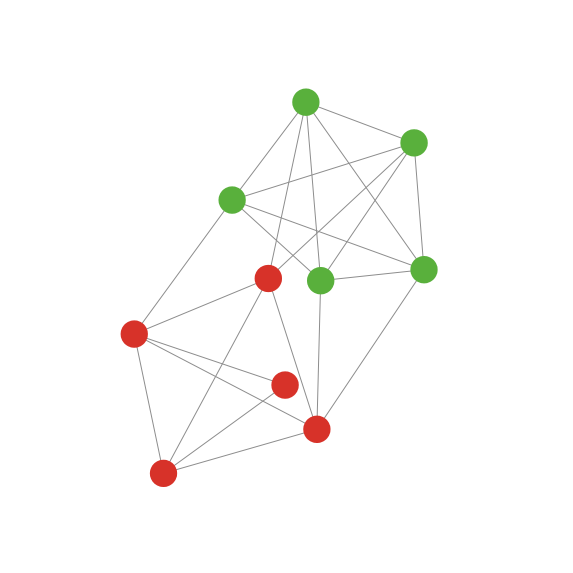
\includegraphics[width=0.8\linewidth]{../Figures/BonusGameViolating.png}
  \caption{\label{fig:bonusviolating} Simulation when the cost of insuring a link is just below the limits. }
\end{figure}


\subparagraph{Consequences of not reaching required number of edges}
Both of these scenarios ends up in a situation where the nodes reach their maximum node degree and therefore receive the bonus. However sometimes nodes take a risk of connecting to other nodes without being able to reach their required number of connections. This means that in certain situation one might end up getting a total $i<m$ connections which results in a much lower payoff than expected. If the variables are set close to a worst-case, such as in table \ref{tbl:maxdegrevalueswitherror} , we end up with two cliques with payoffs close too or worse than the payoff each node had initially. 

\begin{table}[h]
\centering
\begin{tabular}{lc}
 \hline
  $\alpha=10,
  \beta=10,
  I_{o}=5,
  I_{l}=11,
  r=8,
  \gamma=25,
  m=8
  $
  \\
  \hline
\end{tabular}
\caption{Parameters used in simulation \label{tbl:maxdegrevalueswitherror}}
\end{table}

With the variables from table \ref{tbl:maxdegrevalueswitherror} the resulting payoffs from figure \ref{fig:bonusviolatingWithErrors} equals $6$ for each of the non-insured nodes and $-1$ for the insured nodes. In comparison, the same figure using the variables from table \ref{tbl:maxdegrevalues} results in a positive payoff $15$ for each of the nodes in the insured clique. This comparison shows the consequences of failing to achieve the required amount of connections, which might be the case if a company is trying to complete a project which requires too many external suppliers. 

\begin{figure}[h]
\centering
  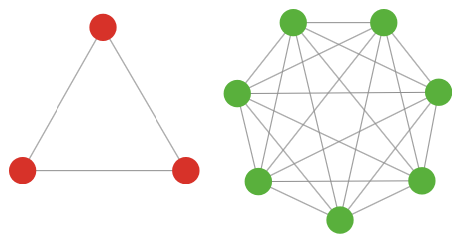
\includegraphics[width=0.6\linewidth]{../Figures/BonusGameInsuredCliqueWithErrors.png}
  \caption{\label{fig:bonusviolatingWithErrors} Simulation when the cost of insuring a link is just below the limits and the maximum node degree is high. }
\end{figure}

\subsection{Game including bulk insurance discount}
Businesses often interpret a quantum discount when purchasing multiple products. From convenience stores we are used to the slogan "buy one get one for free". This is also widely used in insurance, for example travel insurances often give discount for adding family members to the same insurance product. Therefore it is likely that insurance companies will offer a quantum discount when a company is insuring more than one connection. How insurance companies choose to formulate their discount rate might vary among the companies. One solution might be to follow a strict 5$\%$ discount per new connection, or let the discount follow a power law. However, we choose to follow a discount rule which reflects the number of connections the company have established. 
The price for adding a new connection will follow the equation:

\begin{equation}
\frac{I_{l}}{i+1}
\label{eq:discount0}
\end{equation}

Here, $i$ is the current number of established connections. This means that the more connections a company acquire the cheaper the connections will be. 
If we add the new rule to the equation \ref{eq:itoi} which shows the connection between two insured nodes, we get the following equations: 

\begin{equation}
    U_{i+1}= 
\begin{cases}
    \alpha + \beta - I_{0} - I_{l},& \text{if } i = 0\\
    U_{i}+\beta -\frac{I_{l}}{i+1},& \text{if }  i>0\\
    U_{i}+\beta -\frac{I_{l}}{i+1}+\gamma,& \text{if } i=m
    
\end{cases}
\label{eq:discount1}
\end{equation}

As described, for insured nodes to connect to each other, $U_{i+1} > U_{i}$. Building on the already existing model, the quantum discount slightly changes the decision process:
\begin{eqnarray}
U_{i}+\beta-\frac{I_{l}}{i+1}+\frac{\gamma}{m-i}&>U_{i} \nonumber \\ 
\beta-\frac{I_{l}}{i+1}+\frac{\gamma}{m-i}&>0 \nonumber \\ 
\beta (i+1)+\frac{\gamma}{m-i}&>\frac{I_{l}}{i+1} \nonumber \\
\llap{$\rightarrow$\hspace{50pt}}  \beta (i+1)+\frac{\gamma (i+1)}{m-i}&>I_{l}
\label{eq:discount2}
\end{eqnarray}

Similar calculation can be done for the other three scenarios in the game, and they all result in almost the same outcome. First of all results from having quantum discounts on new connections results in a overall higher payoff for the nodes, as long as $i>1$. Since the cost of insuring a new link becomes cheaper. This means that the nodes will have a higher incentive to create links to each other, because the left side of equation \ref{eq:discount2} yields a higher payoff than before. Which leads to a consequence that more insured nodes could connect to non-insured nodes. 
Building on the final condition \ref{eq:final-insurance-clique-condition} in previous section, we now get:

\begin{eqnarray}
\beta+\gamma-r<\frac{I_{l}}{i+1}<\beta+\frac{\gamma}{m} \nonumber \\
\beta(i+1)+\gamma(i+1)-r(i+1)<I_{l}<\beta(i+1)+\frac{\gamma(i+1)}{m}
\label{eq:final-insurance-clique-condition-with-discount}
\end{eqnarray}

SJEKK OM \ref{eq:final-insurance-clique-condition-with-discount} stemmer.... 
From equation \ref{eq:final-insurance-clique-condition-with-discount} we see that the initial variable $I_(l)$ has to be priced higher, in order to ensure that only insured nodes connects to other insured nodes (STEMMER DETTE???). However, beside this drawback, we also experience some positive effects from the modification, since the the purchase of more connections is cheaper the product might be more attractive for potential customers. 
\section{Model 2b: Model with incomplete information}
\label{Model with incomplete information}
Although, we previously mentioned that we chose to assume complete information about other nodes type. We wanted to get an impression of the complexity when modeling a scenario where some nodes lack information about the other nodes type. The way we model this is by letting nature selecting whether a player is insured or not, a node is insured with probability $p$, and not insured with probability $1-p$. 
All nodes know their own type, but in the link establishment process only one node knows the type of the other. The other node only know the probability of the other node being insured or not. 
We want to see if it is possible for the nodes with incomplete information to distinguish an insured node from a non-insured one, and then be able to follow the same procedures as in the other nodes. 
\subsection{Analysis}
When facing a game like this, there exists two types of equilibriums, one where node 2 is able to seperate node 1's type, called separating equilibrium. The other is where he is not able to separate them, called pooling equilibrium. 
We have two types of node, type 1 $(t1)$: insured and type 2 $(t2)$: not insured. 

\subparagraph{Node 2 is insured.}There are two different games to model, one where node 2 is insured, and the other where he is not insured. We start with the one where he is insured.
Node 1's type is chosen randomly by nature, with probability $p$ of being type 1 and $1-p$ of being type 2.
\begin{figure}[h]
\centering
  \centering
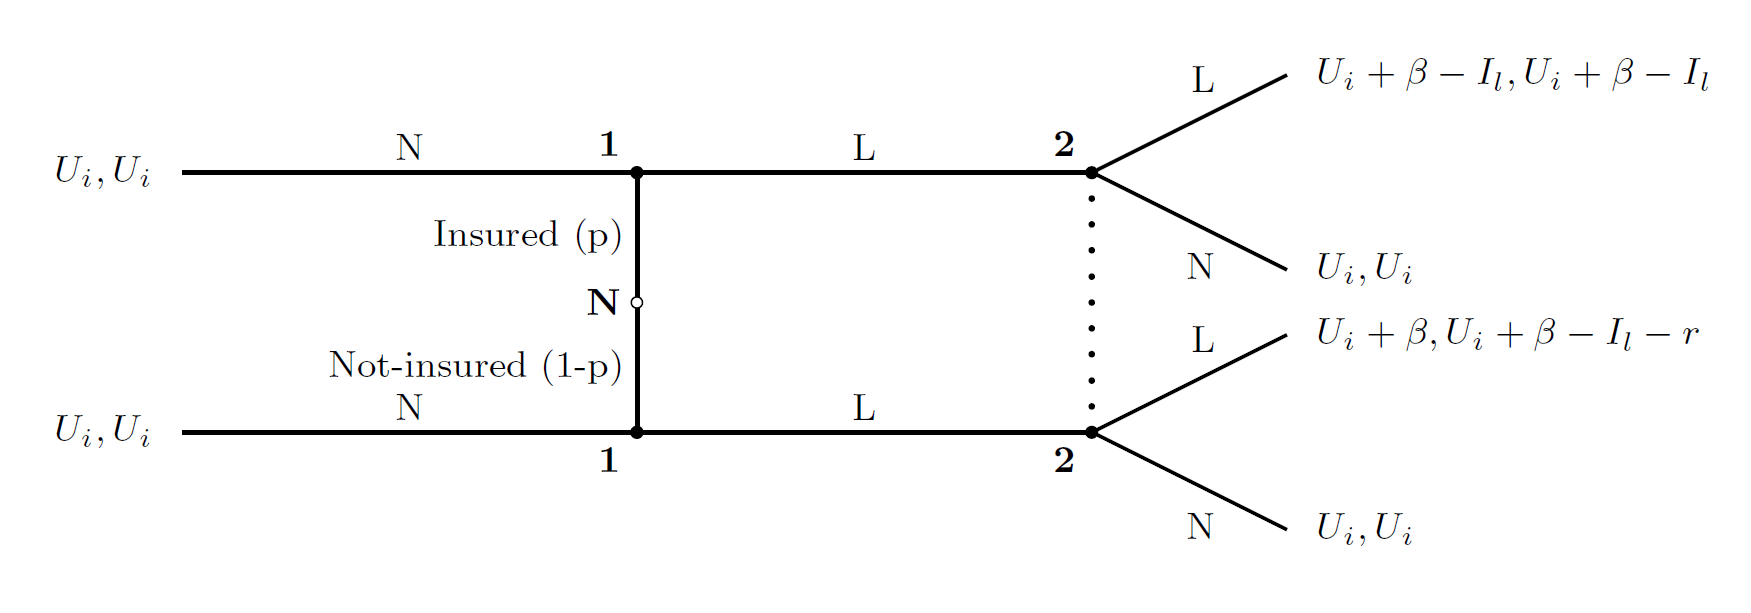
\includegraphics[width=1\linewidth]{../Figures/SignalingGameInsured.png}

\caption{Signalling game with two nodes, node 1's type choosen by nature, node 2 is insured. Node 1 have complete information, node 2 suffer from incomplete information, and act on best response functions based on beliefs. \label{fig:signalingInsured}}

\end{figure}

In the extensive-form shown in Figure \ref{fig:signalingInsured}, we see that $t2's$ strategy L dominates N, and thus $t2$ will never play $N$.
\subparagraph{Separating equilibrium.}
Since node 1 will never play $N$ as type 2, there are only one possible separating equlibrium, type 1 plays $L$ and type 2 plays $N$. Hence node 2's beliefs are as in Eq.(\ref{eq:node2belief}).
\begin{equation}
    \sigma_{1}(t_{i})= 
\begin{cases}
   N,& \text{if } t1\\
   L,& \text{if } t2  
\end{cases}
\label{eq:node2belief}
\end{equation}
Let $\mu_{1}(t_{i} | N )$, denote the probability that node 1 is of type $t_{i}$. By using bayes rule we get this equation:
\begin{equation}
\mu_{1}(t_{1} | N )=\frac{P(N|t_{1})P(t_{1})}{P(N)}=\frac{P(N|t_{1})P(t_{1})}{P(N|t_{1})P(t_{1})+P(N|t_{2})P(t_{2})}
\end{equation}

With node 2's belief, we get that $\mu_{1}(t_{1} | N )=1$ and $\mu_{1}(t_{2} | L )= 1 $. We can now calculate node 2's expected utility from playing L and N:
\begin{eqnarray}
EU_{2}(L,L)=\mu_{1}(t_{1} | L )U_{2}(L,L;t_{1})+\mu_{1}(t_{2} | L )U_{2}(L,L;t_{2}) \nonumber\\
\llap{$\rightarrow$\hspace{50pt}}EU_{2}(L,L)=U_{i}+\beta-I_{l}-r \\
EU_{2}(N,L)=\mu_{1}(t_{1} | L )U_{2}(N,L;t_{1})+\mu_{1}(t_{2} | L )U_{2}(N,L;t_{2})\nonumber\\
\llap{$\rightarrow$\hspace{50pt}}EU_{2}(N,L)=U_{i}
\end{eqnarray}
From these two equations we see that the best response of node 2($BR_2$) when he observes the other node choosing action $L$ is:
\begin{equation}
BR_{2}(L)=
\begin{cases}
L, & \text{if }\beta - r \geq I_{l}\\
N, & \text{if } \beta -r<I_{l}
\end{cases}
\label{eq:insuredBR}
\end{equation}
Node 2's expected utility when type 1 chooses N, is easily seen to be $U_{i}$. 
To confirm if this is a separating equilibrium we must see if node 1 has any incentive to deviate from the strategies in node 2's belief.
Type 2 will never deviate, so lets investigate type 1.
In order to get node 1 to be willing to play N when he knows node 2's best response function, the following must hold: $\beta<I_{l}$. If this is true, then node 2's best response is to play N. I.e. the only separating equilibrium is the following:

\begin{eqnarray}
\beta<I_{l}\\
 \sigma_{1}= 
\begin{cases}
   N,& \text{if } t1\\
   L,& \text{if } t2  
\end{cases}\\
BR_{2}(\sigma_{1})=N
\end{eqnarray} 
This means that in a separating equilibrium, the game will end up with no link establishment.
\subparagraph{Pooling equilibrium.}
In a pooling equilibrium node 2 will not be able to distinguish the two types, and since $t1$'s strategy $L$ dominates $N$, i.e. there is only one possible equilibrium, the one where both types of node 1 plays $L$.
\begin{equation}
    \sigma_{1}(t_{i})= 
\begin{cases}
   L,& \text{if } t1\\
   L,& \text{if } t2  
\end{cases}
\label{eq:node2beliefpooling}
\end{equation}
By using bayes rule we get that $\mu(t_{1}|L)=p$ and $\mu(t_{2}|L)=1-p$.
Node 2's expected utility is then:
\begin{eqnarray}
EU_{2}(L,L)=p(U_{i}+\beta-I_{l})+(1-p)(U_{i}+\beta-I_{l}-r)\nonumber\\
\llap{$\rightarrow$\hspace{50pt}}EU_{2}(L,L)=U_{i}+\beta-I_{l}-r+pr\\
EU_{2}(N,L)=U_{i}
\end{eqnarray}
From this we get node2's best response:
\begin{equation}
BR_{2}(L)=
\begin{cases}
L ,& \text{if } \beta + rp-r\geq I_{l} \\
N ,& \text{if } \beta +rp -r < I_{l} 
\end{cases}
\end{equation}
By using this best response function, node 1 sees that as long as $\beta>I_{l}$ he will never deviate from node 2's beliefs. Hence, it is a pooling equilibrium where both nodes choose $L$, as long as $\beta>I_{l}$ and $\beta +rp-r>I_{l}$.
We also know that: $rp-r\leq0$ is allways true, and thus there also exists a pooling equilibrium where node 1, plays $L$, and node 2, plays $N$. This equilibrium will occur when $\beta>I_{l}$ and $\beta+rp-r<I_{l}$.
\subparagraph{Node 2 not insured.}
Here we will analyze the game when node 2 is not insured.
The rules of the game are as before, the only thing that has changed is the type of node 2, and thus the payoffs are different and we need to see if there exists separating and pooling equilibrium in this game as well.
\begin{figure}[h]
\centering

  \centering
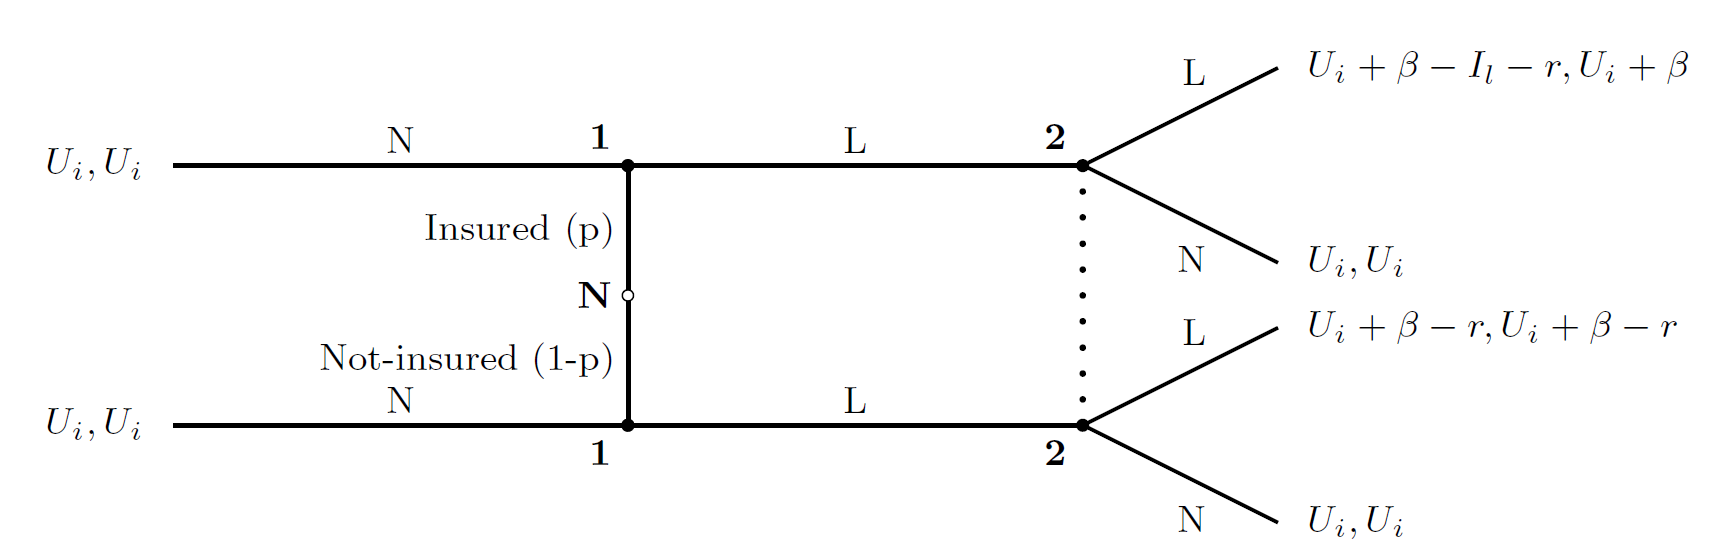
\includegraphics[width=1\linewidth]{../Figures/SignalingGameNotInsured.png}

\caption{Signalling game with two nodes, node 1's type choosen by nature, node2 is not insured. Node 1 have complete information, node 2 suffer from incomplete information, and act on best response functions based on beliefs. \label{fig:signalingNotInsured}}

\end{figure}
\subparagraph{Separating equilibrium.}
In this game there is no dominant strategy for node 1, thus we have to check for the two possible separating equilibriums.
We start with the separating equilibrium with the beliefs shown in Eq.(\ref{eq:node2beliefnotinsured}).
\begin{equation}
    \sigma_{1}(t_{i})= 
\begin{cases}
   L,& \text{if } t1\\
   N,& \text{if } t2  
\end{cases}
\label{eq:node2beliefnotinsured}
\end{equation}
With the beliefs in Eq.(\ref{eq:node2beliefnotinsured}), this is node 2's expected payoffs:
\begin{eqnarray}
EU_{2}(L,L)=(U_{i}+\beta) \\
EU_{2}(N,L)=(U_{i})
\end{eqnarray}
From this we see that his best response when node 1's action is L, is to allways play $L$: \begin{equation}
BR_{2}(L)= L
\end{equation}
To see if this is an equilibrium, we have to see if node 1 has any incentive to deviate. 
We need to check for the two types of node 1:
If $\beta>r$ then type 2 would deviate, because he could achieve a higher payoff by playing $L$, given the beliefs of node 2 in Eq.(\ref{eq:node2beliefnotinsured}). Hence we know that for this to be an equilibrium, the following has to hold
\begin{equation}
\beta < r
\label{eq:sepcondition}
\end{equation}  
When analyzing from node 1 type 1's perspective, for him to play L, this has to hold: $U_{i}+\beta-I_{l}-r > U_{i}$. The only way this can hold is if $\beta>I_{l}+r$. We see that Eq.(\ref{eq:sepcondition}) is violating this condition, and thus we have no separating equilibrium with the beliefs in Eq.(\ref{eq:node2beliefnotinsured}).

Now lets look at the other possible separating equilibrium, see Eq.(\ref{eq:node2beliefnotinsured2}).
\begin{equation}
    \sigma_{1}(t_{i})= 
\begin{cases}
   N,& \text{if } t1\\
   L,& \text{if } t2  
\end{cases}
\label{eq:node2beliefnotinsured2}
\end{equation}
Node 2's expected payoffs are as follows:
\begin{eqnarray}
EU_{2}(L,L)=U_{i}+\beta-r \\
EU_{2}(N,L)=U_{i}
\end{eqnarray}
From this we get the best response function:
\begin{equation}
BR_{2}(L)=
\begin{cases}
L ,& \text{if } \beta\geq r \\
N ,& \text{if } \beta<r 
\end{cases}
\end{equation}
For this to be a separating equilibrium, we need to see if node 1 would deviate from node 2's beliefs. 
Type $t1$ will not deviate as long as $\beta<I_{l}+r$. Type $t2$ will not deviate if $\beta \geq r$, if this condition is true, we see that node 2 will play $L$. I.e. the only separating equilibrium that exists is when node 2 plays $L$, node 1 of type $t1$ plays $N$ and node 1 of type $t2$ plays $L$.
For this to happen we get this condition on $\beta$. \begin{equation}
I_{l}+r>\beta>r
\label{eq:conditionseparatingequilibrium}
\end{equation}
\subparagraph{Pooling equilibrium.}
Two possible, one where both types of node 1 plays $L$, and one where both types plays $N$. Lets first analyze the one where both types of node 1 plays $L$.
\begin{equation}
    \sigma_{1}(t_{i})= 
\begin{cases}
   L,& \text{if } t1\\
   L,& \text{if } t2  
\end{cases}
\label{eq:node2beliefnotinsuredpooling}
\end{equation}
With the beliefs shown above, node 2's expected payoffs are: \begin{eqnarray}
EU_{2}(L)=p(U_{i}+\beta)+(1-p)(U_{i}+\beta-r) \nonumber \\
EU_{2}(L)=U_{i}+\beta-r+pr \\
EU_{2}(N)=U_{i}
\end{eqnarray}
From this we get the best response function :
\begin{equation}
BR_{2}(L)=
\begin{cases}
	L,& \text{if } \beta\geq r-pr\\
   N,& \text{if } \beta<r-pr  
\end{cases}
\end{equation}
Will node 1 deviate knowing this?
Type $t1$ will not deviate as long as: $\beta - I_{l} \geq r$, and type $t2$ will not deviate as long as $\beta >r$.
From this we get the final condition, if $\beta-I_{l}\geq r$ then there exists a pooling equilibrium where both types of node 1 plays $L$ and node 2 also play $L$.
From this we see that the other pooling equilibrium where both types of node 1, plays $N$, will only occur when $\beta<r \text{ and } \beta<I_l+r$.

\subparagraph{Result and findings.}
When one player lack knowledge about the other player, we were only able to find two scenarios where he could separate the two types of the other node. This is possible when player 2 is insured and $\beta<I_{l}$. He can then separate the insured and non-insured types of the other node, because it is only the non-insured node who would want to establish link. Since $\beta<I_{l}$ his best response is to not establish any link.

The other scenario where the node with incomplete information are able to separate is when he is not insured, and $r<\beta<I_{l}+r$. In this scenario it is only the non-insured node who would want to establish a link. Thus in this scenario the game will end up with a link between two non-insured nodes.

We where also able to find some pooling equilibriums, if the node with incomplete information is insured, a link will be established if $\beta+rp-r>I_{l}$. However, if $I_{l}<\beta \text{ but } I_{l}>\beta+rp-r$, then the pooling equilibrium will be that node 1 wants to establish link, but node 2 rejects.
A pooling equilibrium where both nodes want to establish a link, occur when node 2 is not insured and $\beta-I_{l}>r$. If $\beta<r$ there will be a pooling equilibrium where both players choose not to establish link. 

What this shows us is that when one player suffer from incomplete information, it is no longer possible for the insurer to force a network to evolve into a clique of only insured nodes. It will also be harder to establish links, because one player must act on beliefs.  
Therefore, we chose not to include the simulation of this model, since the result would only be a clique of non-insured or a giant clique of every node. 


\section{DETTE ET ANNET STED KANSKJE? BLIR LITT RART Å HOPPE INN I DET HER}
By adjusting the parameter one can assure that only insured agents connects to other insured agents, and the opposite,
that only uninsured agents connects to each other. Hence as we can see from the figure \ref{fig:fincont} clustered
networks of insured agents (red) are created, and  as the paper \cite{contagion} showed, these clustered trusted
networks, can achieve higher, super-critical, payoff by increasing their node degree past the critical point.

\begin{figure}[h]
\centering
\begin{subfigure}{.5\textwidth}
  \centering
  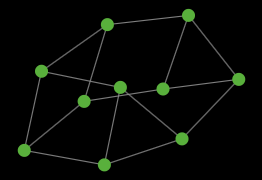
\includegraphics[width=0.8\linewidth]{../Figures/financialContagion1.png}
  \caption{\label{fig:fincont1} Initial graph with 10 agents.}
\end{subfigure}
\quad
\begin{subfigure}{.46\textwidth}
  \centering
  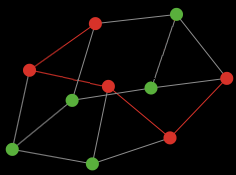
\includegraphics[width=0.8\linewidth]{../Figures/financialContagion2.png}
  \caption{\label{fig:fincont2} Insured agents (red) forms a network}
\end{subfigure}
\caption{\label{fig:fincont} shows how insured agents connects with each other to form a network to achieve super-critical payoffs.}
\end{figure}

, because the nodes can thus receive a super-critical payoff, and they are also insured against contagious risk.  

Figure \ref{fig:GTmodel1equations} presents the individual payoffs in a formation game between two agents in the described model. It is assumed that both agents has to have a desire to establish a connection in order to create a link between them. This is reasonable since a company would not prefer to enter into an agreement with negative expected payoff. As in this case would be the result when an insured agent is requested a connection with someone without insurance. 
 
 
\begin{figure}[h]
\centering
\begin{tabular}{@{}c@{}}
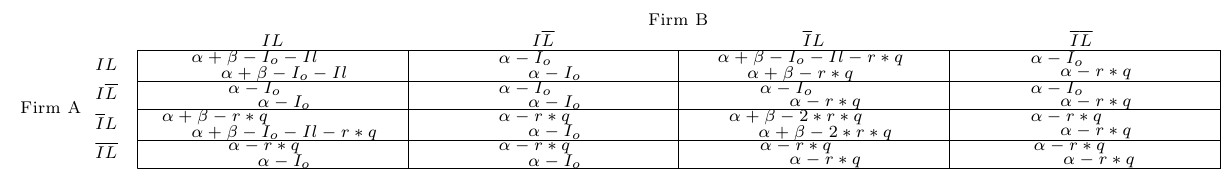
\includegraphics[width=1.0\textwidth]{../Figures/gameTheoryModel1WithEquations.png}
\end{tabular}
\caption[Caption for LOF]{\label{fig:GTmodel1equations} Normal form game between two agents individually choosing to purchase insurance and express desire to connect to the other  \footnotemark }
\end{figure}
\footnotetext{A link will only be created if both agents wishes to establish a connection.}

If we give value to the variables in figure \ref{fig:GTmodel1equations} one can observe the model's different equilibrium's. It is difficult to know exactly how the variables are set and this would vary considerably between different markets. In a real worlds scenario the variables would also be different for each agent. However in figure \ref{fig:GTmodel1} we decided to set a fixed value (which is assumed to be corresponding to the real values) for each variable in order to show a concept of how cyber-insurance can be used to create beneficial payoffs.
The following values where used: $\alpha$ = 10, $\beta$ = 10, $I_{o}$ = 5, $I_{l}$ = 2, $r$  = 20, $q$ = 0.5.


\begin{figure}[h]
\centering
\begin{tabular}{@{}c@{}}
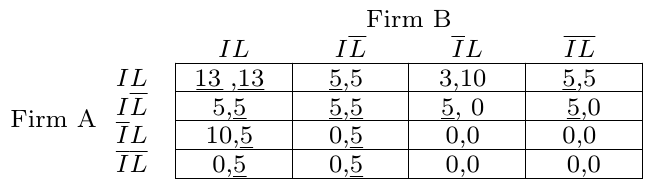
\includegraphics[width=0.6\textwidth]{../Figures/gameTheoryModel1WithNumbers.png}
\end{tabular}
\caption{\label{fig:GTmodel1} Shows equilibrium's in the resulting payoff matrix.}
\end{figure}

From the payoff matrix \ref{fig:GTmodel1} we observe two different Nash equilibrium's: One when both agents are insured and wants to connect to the other agent, and one when both are insured but does not want to establish a connection. These are the possible outcomes between the two agents, however as we can see it the social optimal solution would be for two insured agents to connect with each other, i.e they would both receive a significantly higher payoff. This demonstrates that a cluster of insured nodes would achieve higher payoffs.  

